\begin{figure*}[!tb]
	\centering
	\begin{subfigure}[b]{.675\textwidth}
		\includegraphics[width = \textwidth]{fig/BBS87-1_H87-01-4.jpg}
		\caption{Übersicht}
		\label{fig:BBS87-1_ProfilOst_Foto_Übersicht}
	\end{subfigure}\hfill
	\begin{subfigure}[b]{.30\textwidth}
		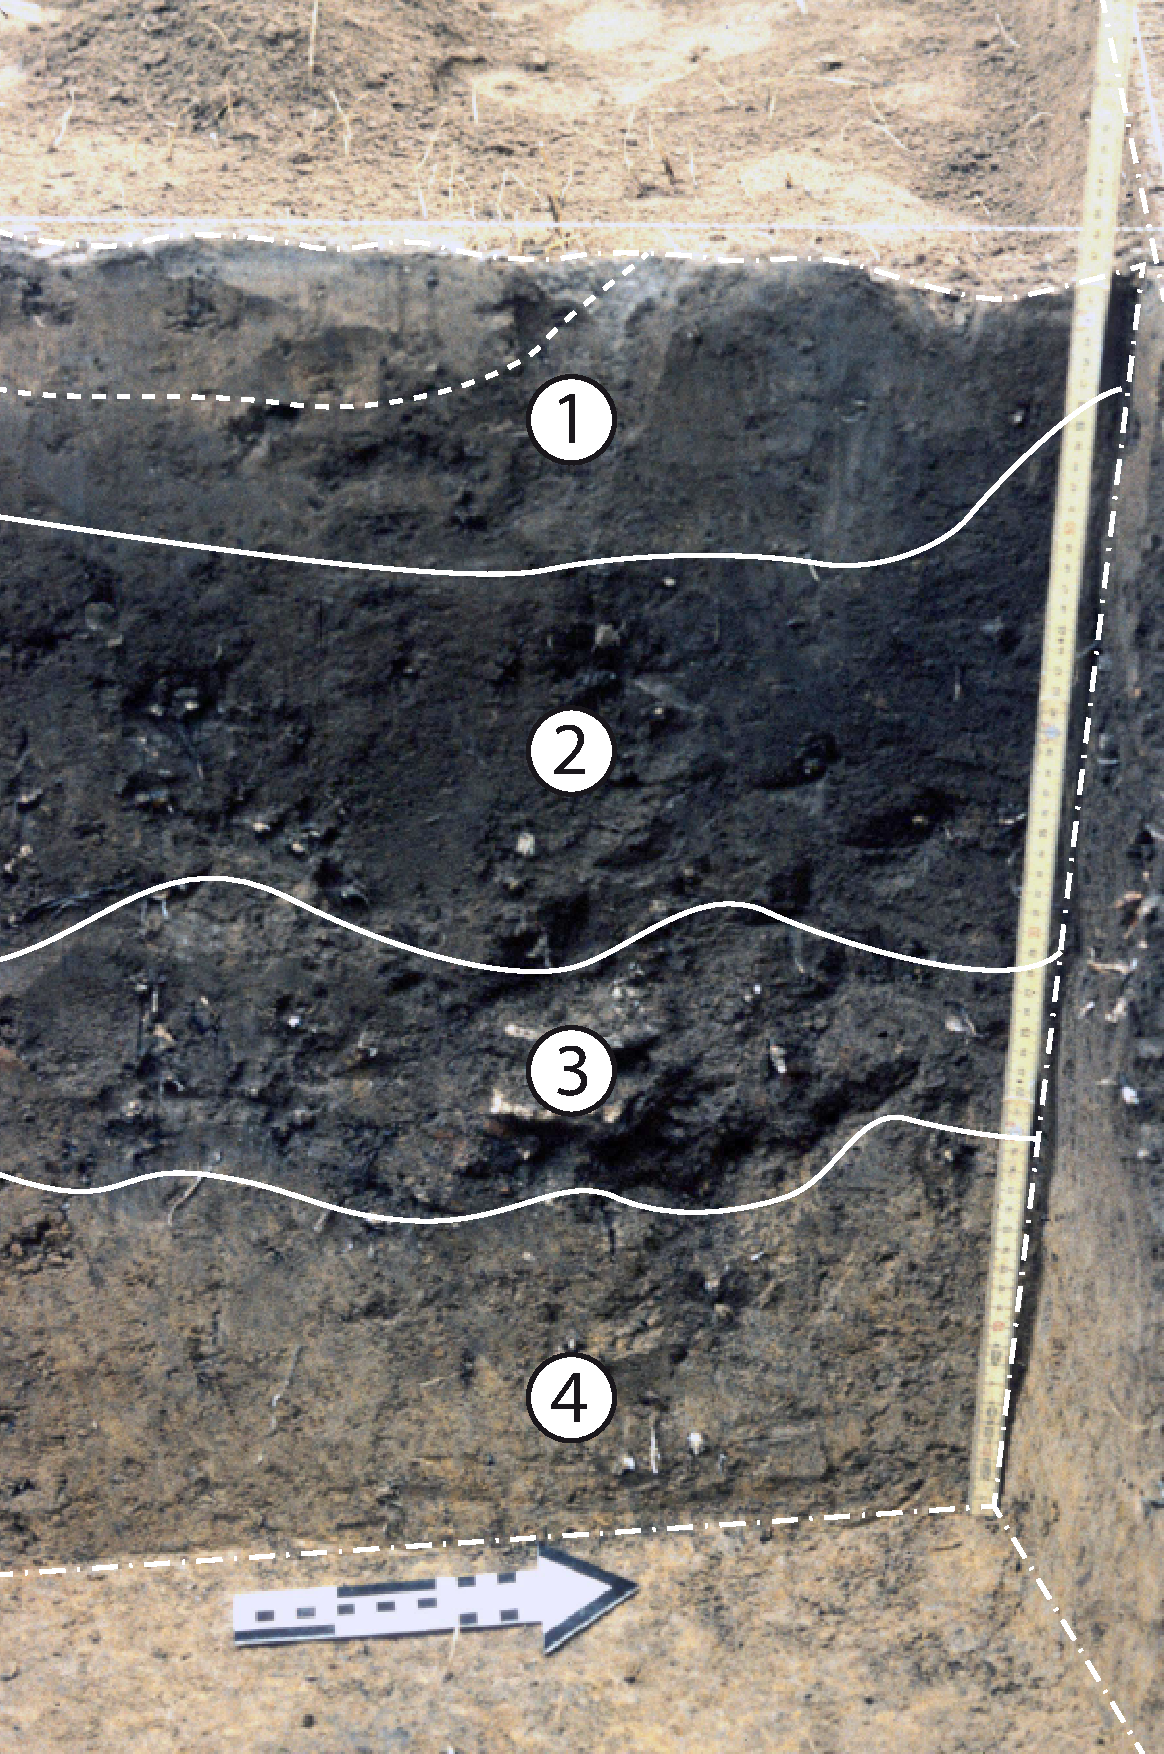
\includegraphics[width = \textwidth]{fig/BBS87-1_H87-01-2.pdf}
		\caption{Nördliche Hälfte}
		\label{fig:BBS87-1_ProfilOst_Foto_Detail}
	\end{subfigure}
	\caption{BBS 87/1: Kontrollprofil zu Beginn der Ausgrabung des 1$\times$1\,m großen Grabungsschnittes. Beide Aufnahmen stellen die einzige vorliegende Dokumentation der beobachteten Profile dar und waren im Original erheblich fehlbelichtet. Sie konnten lediglich bis zum hier abgebildeten Stand aufbereitet werden (Fotos: H. Holsten, 1987).}
	\label{fig:BBS87-1_ProfilOst_Foto}
\end{figure*}

\begin{table*}[tb]
	\centering
	{\footnotesize \begin{sftabular}{@{}lrrrr@{}}
\toprule
   \textbf{Fundkategorie} &  \textbf{Anzahl} &    \textbf{\%} &  \textbf{Gewicht (kg)} &    \textbf{\%} \\
\midrule
 gebrannter Lehm &       6 &   8,0 &          0,10 &  10,2 \\
         Keramik &      67 &  89,3 &          0,77 &  80,0 \\
        Schlacke &       1 &   1,3 &          0,05 &   5,1 \\
          Sonder &       1 &   1,3 &          0,04 &   4,7 \\
\bottomrule
\end{sftabular}
}
	\caption{BBS~87/1: Anteil verschiedener Fundmaterialien.}
	\label{tab:BBS87-1_Funde}
\end{table*}

\section*{\begin{tabular*}{\linewidth}{@{}l @{\extracolsep{\fill}} r@{}}
Nr.~6 & BBS~87/1\\
\end{tabular*} 
}

\textsf{\textbf{Bobusa (\mbox{Sangha}; Fpl.~239)}}

\vspace{1em}

\noindent\begin{tabular}{@{}rl@{}}
\textbf{Feldarbeit:} & \begin{tabular}[t]{@{}l@{}}\textbf{01.05.--03.05.1987}\\ \textbf{(C. Kanimba Misago)}\end{tabular} \\
\textbf{Abb.:} & \textbf{\ref{fig:BBS87-1_ProfilOst_Foto}--\ref{fig:BBS87_1_Funde}} \\
\textbf{Tab.:} & \textbf{\ref{tab:BBS87-1_Funde}}\\
\textbf{Taf.:} & \textbf{33.12--33.15} \\ 
\textbf{Lit.:} & \textbf{--} \\ 
\end{tabular}

\paragraph{Grabung und Befunde}\hspace{-.5em}|\hspace{.5em}%
Das Dorf Bobusa liegt etwa 20\,km nördlich der Mündung des \mbox{Sangha} in den Kongo und bei umfangreichen Prospektionen wurden zwei offene Lehmentnahmegruben entdeckt, in denen sich Keramik fand. Ausgehend von den beiden Gruben wurde jeweils ein 1\,$\times$\,1\,m großer Testschnitt angelegt, der die in den Gruben sichtbare Schicht-Abfolge erfassen sollte. Für den Schnittkasten BBS~87/2 (Kat.-Nr.~7) liegt die Dokumentation des Ausgräbers Hermann Holsten vor, während die Unterlagen zum durch C. Kanimba Misago ausgegrabenen Testschnitt BBS~87/1 verschollen sind. Aus den vorliegenden Fotos, die sämtlich von H. Holsten als Situationsfotos angefertigt wurden, und den Tagebuchnotizen von M.~K.~H. Eggert lässt sich das Folgende rekonstruieren: Im westlichen Teil einer etwa 2--2,5\,m großen und 0,6--0,7\,m tiefen Lehmentnahmegrube wurde ein Profil angelegt, welches zugleich das Ost-Profil des davon ausgehenden Grabungsschnittes BBS~87/1 bildete.\footnote{Das einzige Foto des Ostprofils zeigt dieses nicht in seiner Gänze, sondern lediglich die nördliche Hälfte (Abb.~\ref{fig:BBS87-1_ProfilOst_Foto_Detail}). Das Bild diente wohl der Dokumentation zweier, im Profil steckenden großer -- nicht mehr genau identifizierbarer -- Keramikscherben oder Knochenstücke in Schicht~3, etwa 0,35--0,4\,m unter der Oberfläche.} Im Anschluss an die Dokumentation dieses Profils wurde eine 1\,$\times$\,1\,m große Fläche in drei Abträgen ausgegraben.

Auf Basis aller vorliegenden Informationen können einige Angaben zur stratigrafischen Situation gemacht werden. Das Fundinventar ist mit Abtragsnummern zwischen 1--3 beschriftet worden und auch im benachbarten Befund BBS~87/2 (Kat.-Nr.~7) wurde so verfahren, dass ein Abtrag grob einer im Profil beobachteten Schicht entsprach. Bei der Betrachtung des verfügbaren Detailfotos des Ost-Profils (Abb.~\ref{fig:BBS87-1_ProfilOst_Foto_Detail}) lassen sich drei Fund-Schichten unterscheiden. Eine dunkelgraue bis schwarze Schicht~2 liegt zwischen den helleren, grauen Schichten~1 und 3. Dieses Schicht-Paket sitzt wiederum auf dem anstehenden Lehm auf (Abb.~\ref{fig:BBS87-1_ProfilOst_Foto}: 4). Es kann daher als Hypothese gelten, dass die Funde der drei Abträge die Schichten im Ost-Profil nachzeichnen.

\begin{figure*}[p]
	\centering
	\begin{subfigure}[t]{\textwidth}
		\centering
		\includegraphics[width=\textwidth]{fig/9-6_BBS87-1_VerteilungFunde_R.pdf}
		\caption{Fundmaterial.\vspace{1em}}
		\label{fig:BBS87-1_VerteilungFunde}
	\end{subfigure}
	\begin{subfigure}[t]{\textwidth}
		\centering
		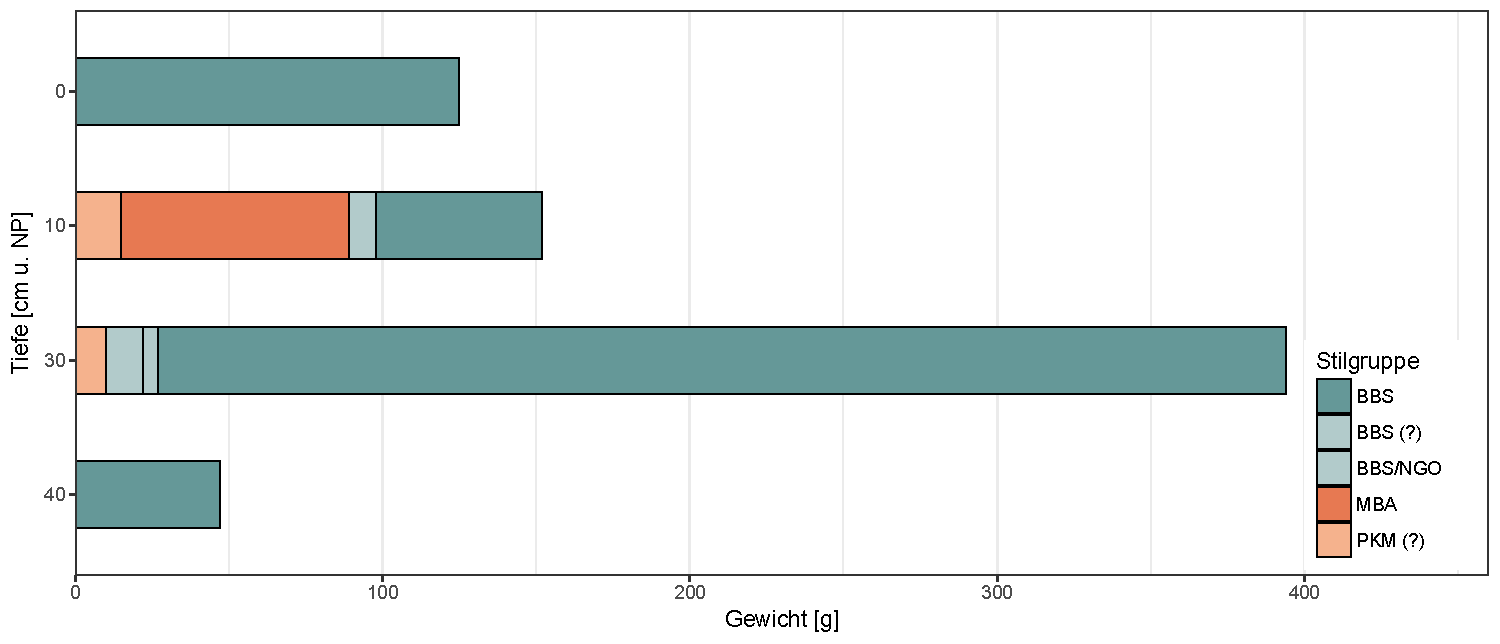
\includegraphics[width=\textwidth]{fig/9-6_BBS87-1_KeramikStilgruppen_R.pdf}
		\caption{Keramische Stilgruppen.\vspace{1em}}
		\label{fig:BBS87-1_VerteilungStilgr}
	\end{subfigure}
	\begin{subfigure}[t]{\textwidth}
		\centering
		\includegraphics[width=\textwidth]{fig/9-6_BBS87-1_Fabrics_R.pdf}
		\caption{\textit{Fabrics}.}
		\label{fig:BBS87-1_VerteilungFabrics}
	\end{subfigure}
	\caption{BBS 87/1: Verteilung der Fundmaterialien (A), keramischen Stilgruppen (B) und \textit{Fabrics} (C) in den entsprechenden Tiefen der Grabung.}
	\label{fig:BBS87_1_Funde}
\end{figure*}

\begin{figure*}[tb]
	\centering
	\includegraphics[width=\textwidth]{fig/9-6_BBS87-1_Fragmentierung_2.pdf}
	\caption{BBS~87/1: Fragmentierungsgrad der Scherben (n~=~67; Größenklassen siehe Anm.~\ref{ftn:Keramik_Fragmentierung}).}
	\label{fig:Fragmenierung_BBS87-1}
\end{figure*}

\vspace{.5em}\noindent Die Grabung erbrachte -- vor dem Hintergrund der geschilderten Rekonstruktion -- den folgenden stratigrafischen Befund (Abb.~\ref{fig:BBS87-1_ProfilOst_Foto}):\footnote{Tiefenangaben beziehen sich auf die rezente Oberfläche und wurden von den Fotos abgenommen (Abb.~\ref{fig:BBS87-1_ProfilOst_Foto}).}
\begin{itemize}[leftmargin=*, labelindent=1em, noitemsep, topsep=0pt]
\item [(1)] 0--0,1\,m; dunkel/leicht grau; heller als (2)
\item [(2)] 0,1--0,3\,m; sehr dunkel/schwarz
\item [(3)] 0,3--0,4\,m; heller als (2); potenziell kompakter beziehungsweise fester als (1) und (2)
\item [(4)] \textgreater\,0,4\,m; anstehender Lehm
\end{itemize}

\paragraph{Keramik\vspace{.5em}}\mbox{}\\
\begin{tabular}{@{}lrl@{}}
Ausgezählt: & 317\,g & \\ 
Bearbeitet: & 451\,g & (59\,\%) \\ 
Insgesamt: & 768\,g & \\ 
\end{tabular} 

\vspace{1em}\noindent Die Grabung BBS~87/101 erbrachte zusammengenommen nur etwas unter 1\,kg Fundmaterial, 80\,\% davon Keramik (Tab.~\ref{tab:BBS87-1_Funde}). Der Großteil stammt aus dem zweiten Abtrag, zwischen 0,1--0,3\,m unter der Oberfläche (Abb.~\ref{fig:BBS87-1_VerteilungFunde}). Es fanden sich keine Stücke, die größer als 70\,$\times$\,70\,mm waren (Abb.~\ref{fig:Fragmenierung_BBS87-1}). Aufgrund des hohen Zerscherbtheitsgrades war eine Stilgruppenansprache nur selten möglich. 

Der Großteil des keramischen Inventars sind formal kaum diagnostische Merkmale aufweisende Scherben mit Schamott-Magerung (87\,\%), die der Bobusa-Gruppe zugerechnet werden (Kap.~\ref{sec:BBS-Gr}). Im ersten, Schicht~1 repräsentierenden Abtrag fand sich das Fragment eines stark bauchigen Gefäßes mit gekehlter Schulter, das dem Mbandaka-Stil des Inneren Konogbeckens \parencite[139--143; Kap.~\ref{sec:MBA-Gr}]{Wotzka.1995} zugerechnet werden kann. Fragmente einer kleinen, rundbauchigen Flasche mit gekehlter Schulter und langem Kegelhals sind ebenfalls der Mbandaka-Gruppe zuzurechnen (Taf.~33.15). Beide Stücke weisen eine auffällige Schamott-Magerung auf. In technischer Sicht unterschieden sie sich nicht vom sonstigen Material aus Bobusa. Im Material des ersten Abtrages befinden sich auch zwei Scherben, die stilistisch wie technisch an die Pikunda-Munda-Gruppe (Kap.~\ref{sec:PKM-Gr}) erinnern.\footnote{Beide Stücke weisen neben horizontalen Rillen auch Wiegebandverzierung auf. Letztere konnte auf Schamott-gemagerter Keramik bislang nicht beobachtet werden. Eines der Stücke ist ein leicht konvexer, ausbiegender Rand, während das zweite Stück das Fragment eines Gefäßes mit gerader oder leicht konvexer Schulter ist.} GE ohne Schamott-Magerung sind kaum vertreten. Eine stratigrafische Abfolge der keramischen Stilgruppen innerhalb der Schichten, welche im Sinne einer chronologischen Gliederung interpretiert werden könnte, kann aus dem vorliegenden Material nicht abgeleitet werden.

\paragraph{Sonstige Funde}\hspace{-.5em}|\hspace{.5em}%
An der Oberfläche fand sich ein keramischer Flaschenstöpsel (Taf.~33.13) und im zweiten, die Schicht~2 repräsentierenden Abtrag ein kantiges Stücke metallisch graulicher, kompakter Schlacke (Abb.~\ref{fig:BBS87-1_VerteilungFunde}).

\paragraph{Datierung}\hspace{-.5em}|\hspace{.5em}%
Das Fundinventar des Schnitts BBS~87/1 setzt sich größtenteils aus dem gegenwärtig nicht direkt zu datierenden Bobusa-Stil zusammen (Kap.~\ref{sec:BBS-Gr}). Lediglich aufgrund loser morphologischer, ornamentaler sowie technischer Ähnlichkeiten lässt es sich in Relation zur Keramik von der gegenwärtig nicht hinreichend ausgewerteten Fundstelle Île des Mimosas im Stadtgebiet von Kinshasa setzen \parencite[siehe][279\,f.]{Eggert.1984}. Die dortigen Funde sind auf Basis einer Radiokohlenstoffdatierung in das 2. bis 4.~Jh. n.~Chr. datiert. Daneben finden sich Vertreter des Pikunda-Munda-Stils (Kap.~\ref{sec:PKM-Gr}) sowie der in die Jüngere Eisenzeit datierenden Stile Mbdandaka (Kap.~\ref{sec:MBA-Gr}) und -- unter Vorbehalt -- Ngombe (Kap.~\ref{sec:NGO-Gr}; Abb.~\ref{fig:BBS87-1_VerteilungStilgr}). 

\paragraph{Interpretation}\hspace{-.5em}|\hspace{.5em}%
Aufgrund des Fehlens der Dokumentation lassen sich nur auf indirektem Wege Rückschlüsse auf die angetroffene Befundsituation ziehen. Eine Deutung der beobachteten Schichten ist auf dieser Basis nicht möglich.